\documentclass{standalone}
\usepackage{pgfplots}
\pgfplotsset{compat=1.17}
\usepackage{amssymb}

\definecolor{tab_blue}{HTML}{1F77B4}
\definecolor{tab_orange}{HTML}{FF7F0E}

\begin{document}
    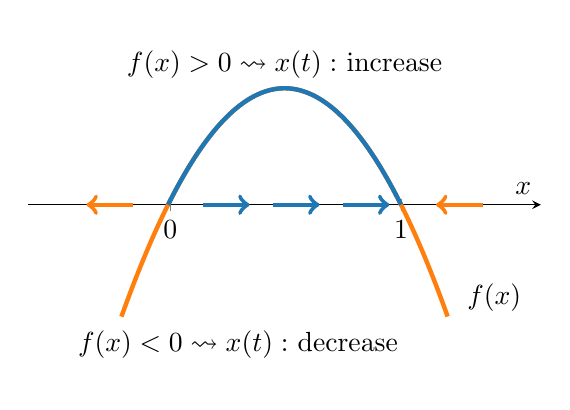
\begin{tikzpicture}[baseline=(current axis.center)]
        \begin{axis}[
            scale=0.95, % scale
            xmin=-0.6,xmax=1.6,ymin=-0.38,ymax=0.38, % range of plot
            % legend style={at={(axis cs: 1,0)}, anchor=south east}, % position of legends
            unit vector ratio = {1, 2}, % aspect ratio
            axis lines = middle, % middle or box
            %axis x line = bottom, % top, middle, bottom, none: axis x line* = ... removes arrow heads
            %axis y line = left, % left, center, right, none: axis y line* = ... removes arrow heads
            xlabel = {$x$}, % axis labels 
            xtick = {0.01, 1},
            xticklabels = {$0$, $1$},
            y axis line style = {draw=none},
            ytick = {-10},
        ]
            \addplot[color=tab_orange, samples=100, domain=-0.2:1.2, ultra thick] {-x^2+x};
            \addplot[color=tab_blue, samples=100, domain=0:1.0, ultra thick] {-x^2+x};
            \node at (0.5, 0.30) {$f(x)>0 \leadsto x(t):$ increase};
            \node at (0.3, -0.30) {$f(x)<0 \leadsto x(t):$ decrease};
            \node at (1.4, -0.20) {$f(x)$};
            \draw[->, color=tab_blue, ultra thick] (0.15,0) -- (0.35,0);
            \draw[->, color=tab_blue, ultra thick] (0.45,0) -- (0.65,0);
            \draw[->, color=tab_blue, ultra thick] (0.75,0) -- (0.95,0);
            \draw[->, color=tab_orange, ultra thick] (-0.15,0) -- (-0.35,0);
            \draw[->, color=tab_orange, ultra thick] (1.35,0) -- (1.15,0);
            
        \end{axis}
    \end{tikzpicture}
    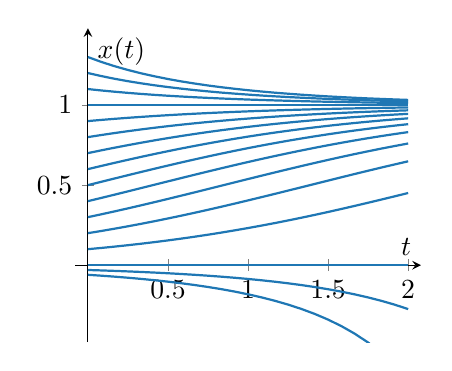
\begin{tikzpicture}[baseline=(current axis.center)]
        \begin{axis}[
            scale=0.7, % scale
            xmin=-0.08,xmax=2.08,ymin=-0.48,ymax=1.48, % range of plot
            % legend style={at={(axis cs: 1,0)}, anchor=south east}, % position of legends
            unit vector ratio = {1, 1}, % aspect ratio
            axis lines = middle, % middle or box
            %axis x line = bottom, % top, middle, bottom, none: axis x line* = ... removes arrow heads
            %axis y line = left, % left, center, right, none: axis y line* = ... removes arrow heads
            xlabel = {$t$}, ylabel = {$x(t)$}, % axis labels 
            declare function={
                sol(\x,\init) = 1/(1 - (1-1/\init)*exp(-\x));
            }
            ]
            % \addplot[thick, color=tab_blue, domain=0:2.0] {1/(1 - exp(-x-3.0))};
            \addplot[thick, color=tab_blue, domain=0:2.0] {0.0};
            \addplot[thick, color=tab_blue, domain=0:2.0] {1.0};
            \pgfplotsforeachungrouped \init in {-0.06, -0.03, 0.1, 0.2, 0.3, 0.4, 0.5, 0.6, 0.7, 0.8, 0.9, 1.1, 1.2, 1.3}{
                \edef\doplot{\noexpand 
                    \addplot [thick, color=tab_blue, domain=0:2.0] {
                        {sol(x,\init)}
                    };
                }
                \doplot
            }
        \end{axis}
    \end{tikzpicture}
\end{document}